\documentclass[a4paper]{article}
\usepackage[dutch]{babel}
\usepackage{color}
\usepackage{geometry}
\usepackage[utf8]{inputenc}
\usepackage{hyperref}
\usepackage{listings}
\usepackage{graphicx}
\usepackage[x11names, rgb, html]{xcolor}

% font
\usepackage{DejaVuSans}
\renewcommand*\familydefault{\sfdefault}
\usepackage[T1]{fontenc}

% Define listing code styles
\definecolor{codegreen}{rgb}{0,0.6,0}
\definecolor{codegray}{rgb}{0.5,0.5,0.5}
\definecolor{codepurple}{rgb}{0.58,0,0.82}
\definecolor{backcolour}{rgb}{0.95,0.95,0.92}

\lstdefinestyle{codestyle}{%
    backgroundcolor=\color{backcolour},
    commentstyle=\color{codegreen},
    keywordstyle=\color{magenta},
    numberstyle=\tiny\color{codegray},
    stringstyle=\color{codepurple},
    basicstyle=\footnotesize,
    breakatwhitespace=false,
    breaklines=true,
    captionpos=b,
    keepspaces=true,
    numbers=left,
    numbersep=5pt,
    showspaces=false,
    showstringspaces=false,
    showtabs=false,
    tabsize=4
}

\lstset{style=codestyle}

% dimensions
\geometry{left=3cm, top=3cm, right=3cm, bottom=3cm}

% hyperlinks
\hypersetup{
  colorlinks=true,
  linkcolor=blue,
  urlcolor=cyan,
}

% image
\graphicspath{ {img/} }

% lists
\providecommand{\tightlist}{%
\setlength{\itemsep}{0pt}\setlength{\parskip}{0pt}}

% Listings style for Docker
\lstdefinelanguage{rust}{%
  keywords={FROM, RUN, COPY, ADD, ENTRYPOINT, CMD,  ENV, WORKDIR, EXPOSE, LABEL, USER, VOLUME, STOPSIGNAL, ONBUILD, MAINTAINER},
  % keywordstyle=\color{blue}\bfseries,
  identifierstyle=\color{black},
  sensitive=false,
  comment=[l]{\#},
  % commentstyle=\color{purple}\ttfamily,
  % stringstyle=\color{red}\ttfamily,
  morestring=[b]',
  morestring=[b]" % chktex 18
}

% preamble
\title{User Manual}
\author{Tim Visée \& Nathan Bakhuijzen}
\date{October 2018}

\begin{document}

  \pagenumbering{gobble}
  \maketitle
  \begin{figure}[h]
    \centering
    
\includegraphics[width=\linewidth]{cant-touch-this}
  \end{figure}
  \clearpage

  \section{Goal}
  The purpose of this manual is twofold:
  \begin{itemize}
    \tightlist
    \item To inform research how to use the platform to execute experiments and
      conduct research
    \item To inform future developers how to continue developing the platform
  \end{itemize}

  \subsection{Problem Definition}
  \textit{What physical motions are natural, effortless and easy, in order to
    control a computer or other digital device?}

  Questions of this nature can be answered using the \textit{Can't Touch This}
  platform. \textit{Can't Touch This} aims to be a platform for researchers that
  would like to conduct research in the field of touchless computer systems. We
  believe that our platform allows researchers to build a strong foundation for
  the future of touchless control. Giving researchers the opportunity to conduct
  research improves the chance for touchless control of computers only seen in
  futuristic movies and tv shows.

  \subsection{Motivation}
  At the start of the KB-80 minor, students were given a choice in the subject
  of the research. Mister Hani introduced us to a series of subjects, of which
  the LeapMotion project was the most interesting to us. The idea of the
  LeapMotion was to create or extend existing software to enable people to
  control a computer without touching any peripherals, like keyboards and mice.

  \subsection{Background information}
  Research in the field of touchless computer systems is motivated by the desire
  for these systems in sterile environments. For example, surgeons often make
  use of computer systems to aid them during their surgeries by providing
  crucial information such as CT, MRI and X-ray scans. This is where touchless
  computer systems come in. These systems allows surgeons on control a computer
  without the need for physical peripherals.
  \clearpage

  \section{Installation Guide}
  \subsection{Requirements}
  \begin{itemize}
    \tightlist
    \item A computer with the Windows (7+), OSX (10.7+, Lion+) or
      Linux (kernel 2.6.18+) operating system
    \item An installation of the LeapMotion
      \href{https://developer.leapmotion.com/sdk/v2}{SDK}
    \item An installation of the
      \href{https://rustup.rs}{Rust} programming language
    \item The physical LeapMotion device itself
  \end{itemize}

  \subsection{Software Dependencies}
  The \textit{Can't Touch This} platform is written using the
  \href{https://rust-lang.org}{Rust programming language}. This means that the
  operating system that the platform will run on must support the Rust language.
  Fortunately, Rust runs on all popular operating systems today, shown above in
  the list of requirements. An up-to-date list of all supported versions can be
  found on the
  \href{https://forge.rust-lang.org/platform-support.html}{Rust website}.
  Additonally, the \textit{Can't Touch This} platform requires the LeapMotion
  \href{https://developer.leapmotion.com/sdk/v2}{SDK} to provide all necessary
  sensor data. Just like the Rust programming language, the LeapMotion SDK can
  be installed on all platforms.

  \subsection{External resources}
  \textit{Can't Touch This} requires no addional resources to run the platform,
  other than the items listed above.

  \subsection{External development tools}
  Continuing development of the \textit{Can't Touch This} platform requires
  basic tools like a text editor or IDE, and a terminal. It is highly
  recommended to use \href{https://git-scm.com/}{git}, as this was used during
  development of the platform. Additionally, setting up an CI server may prove
  useful. Setting up an CI server is beyond the scope of this manual.
  \clearpage

  % 2. User instructions
  % Step by step instructions on how to use the research platform to conduct
  % research.
  % Checklist:
  %   •	Instructions to run the experiment (explained in build plan)
  %   •	Aimed at non technical researchers
  %   •	Include screenshots when possible

  % Bonus points: make a video of the instructions, upload to youtube and
  % include link in manual
  % Note: even if video instructions are created the manual should still have
  % written instructions
  \section{User Instructions}
  This chapter gives users instructions on how to use the \textit{Can't Touch
    This} platform. It assumes that the user has followed the instructions found
  in the \textit{Installation} chapter. The following instructions will detail
  how to setup the platform so that you can conduct the \textit{experiments}
  found later in this manual.
  % TODO: Write detailed instructions on how to run the experiments

  \subsection{Usage}
  \begin{itemize}
    \tightlist
    \item Attach the LeapMotion device using it's provided USB cable
    \item Start the LeapMotion tracking program provided by the LeapMotion SDK
    \item Start the \textit{Can't Touch This} platform by running the provided
      executable program, or run it manually in a terminal (\verb_cargo run_)
    \item Start up an web browser (Chrome, Firefox, Safari, etc) and navigate to
      \\ \url{http://localhost:8000}
    \item Click on '\textit{Start Recording}'
    \item Move your physical hand above the LeapMotion device to make a desired
      gesture
    \item Once you are done making the gesture, click on
      '\textit{Stop Recording}'
    \item The recorded gesture you've just made should be visibly represented on
      the canvas
    \item Save the gesture by clicking on '\textit{Save Recording}' and bind the
      gesture to a predefined action
    \item Click on '\textit{Recognition Mode}' and make one of the gestures
      you've made beforehand
    \item The computer will give positive feedback if the gesture is recognized
  \end{itemize}
  \clearpage

  \section{Requirements}
  This chapter details the list of open and finished requirements of the
  \textit{Can't Touch This} platform. The prioritization of this list is not
  according to the MoSCoW method. This is because this exclusive project
  required us to figure out what to do on the fly, rather than planning
  everything out beforehand.

  Requirements that are satisfied: 
  \begin{itemize}
    \tightlist
    \item An Operating System independant platform
    \item A web interface for users
    \item A list of predefined gestures
    \item The ability to record and store new gestures
    \item The ability to use fingers of both hands in a gesture
  \end{itemize}
  By using the Rust programming language we inherently met the Operating System
  requirement. This saved us a lot of work and allowed us to focus on the
  platform's functionality. Similarly, we chose to use a web interface for the
  interaction between user and system. This also saved us a substantial
  workload.

  Requirements that are still open:
  \begin{itemize}
    \tightlist
    \item The ability to bind actions to predefined or recorded gestures
    \item The ability to combine multiple sensors
  \end{itemize}
  The ability to bind actions to gestures is unfinished because of two reasons.
  The first reason is a lack of time. Writing \textit{Can't Touch This} from
  scratch is a large task, and it consumed most of our development time. Second,
  executing actions based on gestures was not the main goal of the platform. The
  goal of the platform is to allow researchers to conduct experiments in the
  field of touchless computer systems. This research is not aided by the ability
  to execute actions based on gestures, but rather on if a gesture is
  recognized at all. It is because of this that we decided to give visual
  feedback in the web interface instead.

  At the start of the project we wanted to combine multiple LeapMotion sensors
  in order to achieve increased accuracy. We looked into this, but we found out
  that this was impossible, due to the proprietary nature of the LeapMotion
  sensor. Several websites pointed out something like this would be better
  suited for the developers of the LeapMotion.
  \clearpage

  % 4. Software Architecture Diagram
  % 4.1 Context view
  % Describe the relationships, dependencies, and interactions between the
  % system and its environment (the people, system.. and external entities with
  % which it interacts). Your system in this view is represented by a blackbox
  % interacting with external entities. See example in Figure 1.
  % 4.2 Functional view
  % Describe the system’s runtime functional elements and their responsibility,
  % interfaces and primary int

  % Figure 1. Example of a context view

  % methodology:
  %   •	Represent each subcomponent of the system with a box in the figure. 
  %   •	Link the system subcomponents with connectors. These connectors define
  %     the interaction between the elements that use it. 
  %   •	Under the figure explain each subcomponent, and give:
  %   •	Inputs
  %   •	Outputs
  %   •	What functionality is available
  %   •	How to invoke each functionality (commands, syntax, …etc).
  \section{Architecture Diagrams}
  \begin{figure}[h]
    \caption{Context Diagram}
    \centering
    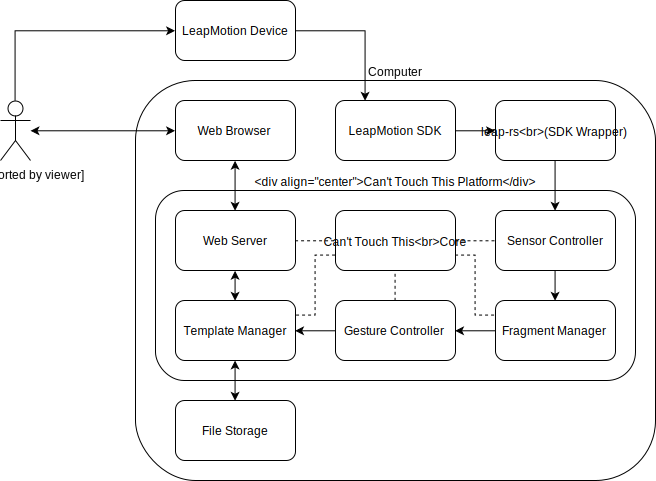
\includegraphics[width=\linewidth]{context-diagram}
  \end{figure}
  In this diagram, the \textit{Can't Touch This} platform displayed globally. It
  Shows three main objects:
  \begin{itemize}
    \tightlist
    \item The user
    \item The LeapMotion device
    \item The Can't Touch This platform
  \end{itemize}
  The user attaches the LeapMotion device to the computer, installs the platform
  and moves it's hand above the sensor to conduct an experiment. The LeapMotion
  device captures the data of the hand, and passes it on through the LeapMotion
  SDK, to the leap-rs wrapper. This leap-rs wrapper maps all functions made
  available through the LeapMotion SDK to the Rust programming language.
  Normally, a platform like \textit{Can't Touch This} would have to be
  programmed using the C programming language, as this is the language the SDK
  is written in.

  The leap-rs wrapper enables the SDK functionality in our platform, which we
  use in the Sensor Controller. The Sensor controller is our gateway of
  information, of our bits and bytes. The Sensor controller passes this data on
  to the Fragment Manager, which records all data and converts it into Points,
  Rotational Points (\textit{RotPoints}) and Traces of both kind. It even
  improves the recorded points in the trace by sampling them. Sampling is ...
  % TODO: Let Tim write this section

  After the conversion and sampling, the Gesture Controller receives the data
  and compares this to existing gestures, stored in the Template Manager. The
  Template Manager compares the received gesture to the existing ones stores on
  the system. The gestures are saved in text files, as the data is not that
  complex. If the system matches the current gestures with an existing one, it
  will give positive feedback through the web interface. The user will see the
  positive feedback and know that that gesture is working well.

  The web interface also retrieves all the stored gestures for the user to
  review. It can add and delete gestures as the user wants, except the
  pre-defined gestures.

  \begin{figure}[h]
    \caption{Context Diagram}
    \centering
    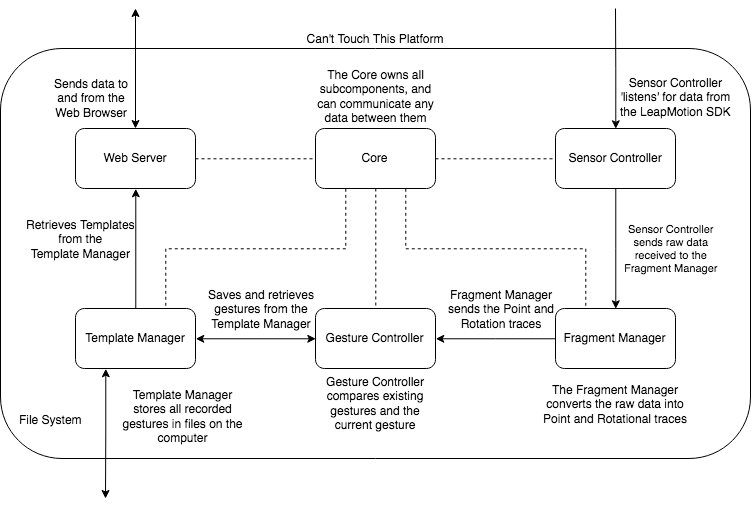
\includegraphics[width=\linewidth]{functional-diagram}
  \end{figure}
  \clearpage

  % 5. Domain model
  % In the domain model you list all:
  %   •	API interfaces
  %   •	Subsystems
  \section{Domain Model}
  \clearpage

  \section{Test Report}
  \subsection{Code Quality} % •	What is the quality of the code
  \subsection{Existing Tests} % •	What has already been tested
  The platform currently has a few unit tests that cover basic operations such
  as the conversion of a \textit{Point} to a \textit{PointTrace} and more. We
  we also have set up a few tests where we cover the comparison of traces, such
  as straight lines and curves. Below you can see the test code:
  \lstinputlisting[
    language=rust,
    caption={%
      Straight line unit test
    },
  ]{code/straight.rs}

  This unit test creates \verb_points_, a trace of \verb_Point3_'s, and compares
  it to \verb_expected_, a \verb_RotTrace_.

  The \verb_PointTrace_ on line 3 contains three points that travel the same
  distance at every step. The platform recognizes this as a straight line, as
  there is no change in the trajectory. the variable \verb_expected_ then gets
  assigned a \verb_RotTrace_ that contains only one \verb_RotPoint_ of 0
  degrees. This is correct, as the line drawn on line 3 is straight.

  \lstinputlisting[
    language=rust,
    caption={%
      Corner unit test
    },
  ]{code/corner.rs}
  The \verb_corner_ test is a little more complicated than the \verb_straight_
  unit test. It creates a \verb_PointTrace_ with points that represent a 2D
  square. The expected RotTrace then contains three \verb_RotPoint_'s of -90
  degrees.

  \subsection{Known Bugs}
  \begin{itemize}
    \tightlist
    \item \textit{Can't Touch This} may crash upon running the release version
      of the exectable
    \item On macOS, the LeapMotion device may never give data to begin with
    \item On macOS, the LeapMotion device may stop recording data randomly
    \item On macOS, the application may not run well when minimalizing the
      backend application
  \end{itemize}
\end{document}
